\documentclass[11pt,addpoints,answers]{exam}

%%%%%%%%%%%%%%%%%%%%%%%%%%%%%%%%%%%%%%%%%%%
% Commands for customizing the assignment %
%%%%%%%%%%%%%%%%%%%%%%%%%%%%%%%%%%%%%%%%%%%

\newcommand{\courseNum}{10-423/10-623}
\newcommand{\courseName}{Generative AI}
\newcommand{\courseSem}{Spring 2024}
\newcommand{\courseUrl}{\url{http://423.mlcourse.org}}
\newcommand{\hwNum}{Homework 4}
\newcommand{\hwTopic}{Multi-Modal Foundation Models}
\newcommand{\hwName}{\hwNum: \hwTopic}
\newcommand{\outDate}{March 13, 2025}
\newcommand{\dueDate}{March 24, 2025}
\newcommand{\taNames}{Abishek, Aravind, Madhura}
\newcommand{\homeworktype}{\string written+prog}
\newcommand{\autograder}{\string yes}
\newcommand{\overleafUrl}{}

%% To HIDE SOLUTIONS (to post at the website for students), set this value to 0: \def\issoln{0}
\providecommand{\issoln}{0}
%\providecommand{\issoln}{1}

%-----------------------------------------------------------------------------
% PACKAGES AND OTHER DOCUMENT CONFIGURATIONS
%-----------------------------------------------------------------------------

\usepackage[margin=1in]{geometry}
\usepackage{amsmath, amsfonts}
\usepackage{enumerate}
\usepackage{graphicx}
\usepackage{titling}
\usepackage{url}
\usepackage{xfrac}
\usepackage{natbib}
\usepackage{amssymb}
\usepackage{amsthm}
\usepackage{paralist}
\usepackage{epstopdf}
\usepackage{tabularx}
\usepackage{longtable}
\usepackage{multirow}
\usepackage{multicol}
\usepackage[colorlinks=true,urlcolor=blue]{hyperref}
\usepackage{algorithm}
\usepackage{algorithmicx}
\usepackage[noend]{algpseudocode}
\usepackage{float}
\usepackage{enumerate}
\usepackage{array}
\usepackage{environ}
\usepackage{times}
\usepackage{textcomp}
\usepackage{caption}
\usepackage{parskip} % For NIPS style paragraphs.
\usepackage[compact]{titlesec} % Less whitespace around titles
\usepackage[inline]{enumitem} % For inline enumerate* and itemize*
\usepackage{datetime}
\usepackage{comment}
% \usepackage{minted}
\usepackage{lastpage}
\usepackage{color}
% \usepackage{xcolor}
\usepackage[dvipsnames]{xcolor}
\usepackage[final]{listings}
\usepackage{tikz}
\usetikzlibrary{shapes,decorations}
\usepackage{framed}
\usepackage{booktabs}
\usepackage{cprotect}
\usepackage{verbatimbox}
\usepackage{multicol}
\usepackage{hyperref}
\usepackage{subcaption}
\usepackage{mathtools} % For drcases
\usepackage{cancel}
\usepackage[many]{tcolorbox}
\tcbuselibrary{listings} % For listings within tcolorbox
\usepackage{soul}
\usepackage[bottom]{footmisc}
\usepackage{bm}
\usepackage{wasysym}
\usepackage{lipsum}

\usepackage{tikz}
\usetikzlibrary{arrows}
\usetikzlibrary{arrows.meta}
\usetikzlibrary{shapes.geometric}
\usetikzlibrary{positioning, arrows, automata, calc}
\usepackage{transparent}
\usepackage{tikz-cd}

%%%%%%%%%%%%%%%%%%%%%%%%%%%%%%%%%%%%%%%%%%%
% Formatting for \CorrectChoice of "exam" %
%%%%%%%%%%%%%%%%%%%%%%%%%%%%%%%%%%%%%%%%%%%

\CorrectChoiceEmphasis{}
\checkedchar{\blackcircle}

\newenvironment{checkboxessquare}{
    \begingroup
    \checkboxchar{$\Box$} \checkedchar{$\blacksquare$} % change checkbox style locally
    \begin{checkboxes}
    }{
    \end{checkboxes}
    \endgroup
    }

    
\newenvironment{oneparcheckboxessquare}{
    \begingroup
    \checkboxchar{$\Box$} \checkedchar{$\blacksquare$} % change checkbox style locally
    \begin{oneparcheckboxes}
    }{
    \end{oneparcheckboxes}
    \endgroup
    }

%%%%%%%%%%%%%%%%%%%%%%%%%%%%%%%%%%%%%%%%%%%
% Better numbering                        %
%%%%%%%%%%%%%%%%%%%%%%%%%%%%%%%%%%%%%%%%%%%

% \numberwithin{equation}{section} % Number equations within sections (i.e. 1.1, 1.2, 2.1, 2.2 instead of 1, 2, 3, 4)
% \numberwithin{figure}{section} % Number figures within sections (i.e. 1.1, 1.2, 2.1, 2.2 instead of 1, 2, 3, 4)
% \numberwithin{table}{section} % Number tables within sections (i.e. 1.1, 1.2, 2.1, 2.2 instead of 1, 2, 3, 4)

%%%%%%%%%%%%%%%%%%%%%%%%%%%%%%%%%%%%%%%%%%
% Custom commands                        %
%%%%%%%%%%%%%%%%%%%%%%%%%%%%%%%%%%%%%%%%%%
\newcommand{\blackcircle}{\tikz\draw[black,fill=black] (0,0) circle (1ex);}
\renewcommand{\circle}{\tikz\draw[black] (0,0) circle (1ex);}

\newcommand{\solo}{ \textcolor{orange}{[SOLO]} }
\newcommand{\open}{ \textcolor{blue}{[OPEN]} }


%%%%%%%%%%%%%%%%%%%%%%%%%%%%%%%%%%%%%%%%%%
% Custom commands for Math               %
%%%%%%%%%%%%%%%%%%%%%%%%%%%%%%%%%%%%%%%%%%
\newcommand{\vc}[1]{\boldsymbol{#1}}
\newcommand{\adj}[1]{\frac{\partial \ell}{\partial #1}}
\newcommand{\chain}[2]{\adj{#2} = \adj{#1}\frac{\partial #1}{\partial #2}}
\newcommand{\ntset}{test}
\newcommand{\zerov}{\mathbf{0}}
\DeclareMathOperator*{\argmin}{argmin}

% mathcal
\newcommand{\Ac}{\mathcal{A}}
\newcommand{\Bc}{\mathcal{B}}
\newcommand{\Cc}{\mathcal{C}}
\newcommand{\Dc}{\mathcal{D}}
\newcommand{\Ec}{\mathcal{E}}
\newcommand{\Fc}{\mathcal{F}}
\newcommand{\Gc}{\mathcal{G}}
\newcommand{\Hc}{\mathcal{H}}
\newcommand{\Ic}{\mathcal{I}}
\newcommand{\Jc}{\mathcal{J}}
\newcommand{\Kc}{\mathcal{K}}
\newcommand{\Lc}{\mathcal{L}}
\newcommand{\Mc}{\mathcal{M}}
\newcommand{\Nc}{\mathcal{N}}
\newcommand{\Oc}{\mathcal{O}}
\newcommand{\Pc}{\mathcal{P}}
\newcommand{\Qc}{\mathcal{Q}}
\newcommand{\Rc}{\mathcal{R}}
\newcommand{\Sc}{\mathcal{S}}
\newcommand{\Tc}{\mathcal{T}}
\newcommand{\Uc}{\mathcal{U}}
\newcommand{\Vc}{\mathcal{V}}
\newcommand{\Wc}{\mathcal{W}}
\newcommand{\Xc}{\mathcal{X}}
\newcommand{\Yc}{\mathcal{Y}}
\newcommand{\Zc}{\mathcal{Z}}

% mathbb
\newcommand{\Ab}{\mathbb{A}}
\newcommand{\Bb}{\mathbb{B}}
\newcommand{\Cb}{\mathbb{C}}
\newcommand{\Db}{\mathbb{D}}
\newcommand{\Eb}{\mathbb{E}}
\newcommand{\Fb}{\mathbb{F}}
\newcommand{\Gb}{\mathbb{G}}
\newcommand{\Hb}{\mathbb{H}}
\newcommand{\Ib}{\mathbb{I}}
\newcommand{\Jb}{\mathbb{J}}
\newcommand{\Kb}{\mathbb{K}}
\newcommand{\Lb}{\mathbb{L}}
\newcommand{\Mb}{\mathbb{M}}
\newcommand{\Nb}{\mathbb{N}}
\newcommand{\Ob}{\mathbb{O}}
\newcommand{\Pb}{\mathbb{P}}
\newcommand{\Qb}{\mathbb{Q}}
\newcommand{\Rb}{\mathbb{R}}
\newcommand{\Sb}{\mathbb{S}}
\newcommand{\Tb}{\mathbb{T}}
\newcommand{\Ub}{\mathbb{U}}
\newcommand{\Vb}{\mathbb{V}}
\newcommand{\Wb}{\mathbb{W}}
\newcommand{\Xb}{\mathbb{X}}
\newcommand{\Yb}{\mathbb{Y}}
\newcommand{\Zb}{\mathbb{Z}}

% mathbf lowercase
\newcommand{\av}{\mathbf{a}}
\newcommand{\bv}{\mathbf{b}}
\newcommand{\cv}{\mathbf{c}}
\newcommand{\dv}{\mathbf{d}}
\newcommand{\ev}{\mathbf{e}}
\newcommand{\fv}{\mathbf{f}}
\newcommand{\gv}{\mathbf{g}}
\newcommand{\hv}{\mathbf{h}}
\newcommand{\iv}{\mathbf{i}}
\newcommand{\jv}{\mathbf{j}}
\newcommand{\kv}{\mathbf{k}}
\newcommand{\lv}{\mathbf{l}}
\newcommand{\mv}{\mathbf{m}}
\newcommand{\nv}{\mathbf{n}}
\newcommand{\ov}{\mathbf{o}}
\newcommand{\pv}{\mathbf{p}}
\newcommand{\qv}{\mathbf{q}}
\newcommand{\rv}{\mathbf{r}}
\newcommand{\sv}{\mathbf{s}}
\newcommand{\tv}{\mathbf{t}}
\newcommand{\uv}{\mathbf{u}}
\newcommand{\vv}{\mathbf{v}}
\newcommand{\wv}{\mathbf{w}}
\newcommand{\xv}{\mathbf{x}}
\newcommand{\yv}{\mathbf{y}}
\newcommand{\zv}{\mathbf{z}}

% mathbf uppercase
\newcommand{\Av}{\mathbf{A}}
\newcommand{\Bv}{\mathbf{B}}
\newcommand{\Cv}{\mathbf{C}}
\newcommand{\Dv}{\mathbf{D}}
\newcommand{\Ev}{\mathbf{E}}
\newcommand{\Fv}{\mathbf{F}}
\newcommand{\Gv}{\mathbf{G}}
\newcommand{\Hv}{\mathbf{H}}
\newcommand{\Iv}{\mathbf{I}}
\newcommand{\Jv}{\mathbf{J}}
\newcommand{\Kv}{\mathbf{K}}
\newcommand{\Lv}{\mathbf{L}}
\newcommand{\Mv}{\mathbf{M}}
\newcommand{\Nv}{\mathbf{N}}
\newcommand{\Ov}{\mathbf{O}}
\newcommand{\Pv}{\mathbf{P}}
\newcommand{\Qv}{\mathbf{Q}}
\newcommand{\Rv}{\mathbf{R}}
\newcommand{\Sv}{\mathbf{S}}
\newcommand{\Tv}{\mathbf{T}}
\newcommand{\Uv}{\mathbf{U}}
\newcommand{\Vv}{\mathbf{V}}
\newcommand{\Wv}{\mathbf{W}}
\newcommand{\Xv}{\mathbf{X}}
\newcommand{\Yv}{\mathbf{Y}}
\newcommand{\Zv}{\mathbf{Z}}

% bold greek lowercase
\newcommand{\alphav     }{\boldsymbol \alpha     }
\newcommand{\betav      }{\boldsymbol \beta      }
\newcommand{\gammav     }{\boldsymbol \gamma     }
\newcommand{\deltav     }{\boldsymbol \delta     }
\newcommand{\epsilonv   }{\boldsymbol \epsilon   }
\newcommand{\varepsilonv}{\boldsymbol \varepsilon}
\newcommand{\zetav      }{\boldsymbol \zeta      }
\newcommand{\etav       }{\boldsymbol \eta       }
\newcommand{\thetav     }{\boldsymbol \theta     }
\newcommand{\varthetav  }{\boldsymbol \vartheta  }
\newcommand{\iotav      }{\boldsymbol \iota      }
\newcommand{\kappav     }{\boldsymbol \kappa     }
\newcommand{\varkappav  }{\boldsymbol \varkappa  }
\newcommand{\lambdav    }{\boldsymbol \lambda    }
\newcommand{\muv        }{\boldsymbol \mu        }
\newcommand{\nuv        }{\boldsymbol \nu        }
\newcommand{\xiv        }{\boldsymbol \xi        }
\newcommand{\omicronv   }{\boldsymbol \omicron   }
\newcommand{\piv        }{\boldsymbol \pi        }
\newcommand{\varpiv     }{\boldsymbol \varpi     }
\newcommand{\rhov       }{\boldsymbol \rho       }
\newcommand{\varrhov    }{\boldsymbol \varrho    }
\newcommand{\sigmav     }{\boldsymbol \sigma     }
\newcommand{\varsigmav  }{\boldsymbol \varsigma  }
\newcommand{\tauv       }{\boldsymbol \tau       }
\newcommand{\upsilonv   }{\boldsymbol \upsilon   }
\newcommand{\phiv       }{\boldsymbol \phi       }
\newcommand{\varphiv    }{\boldsymbol \varphi    }
\newcommand{\chiv       }{\boldsymbol \chi       }
\newcommand{\psiv       }{\boldsymbol \psi       }
\newcommand{\omegav     }{\boldsymbol \omega     }

% bold greek uppercase
\newcommand{\Gammav     }{\boldsymbol \Gamma     }
\newcommand{\Deltav     }{\boldsymbol \Delta     }
\newcommand{\Thetav     }{\boldsymbol \Theta     }
\newcommand{\Lambdav    }{\boldsymbol \Lambda    }
\newcommand{\Xiv        }{\boldsymbol \Xi        }
\newcommand{\Piv        }{\boldsymbol \Pi        }
\newcommand{\Sigmav     }{\boldsymbol \Sigma     }
\newcommand{\Upsilonv   }{\boldsymbol \Upsilon   }
\newcommand{\Phiv       }{\boldsymbol \Phi       }
\newcommand{\Psiv       }{\boldsymbol \Psi       }
\newcommand{\Omegav     }{\boldsymbol \Omega     }

%%%%%%%%%%%%%%%%%%%%%%%%%%%%%%%%%%%%%%%%%%%
% Code highlighting with listings         %
%%%%%%%%%%%%%%%%%%%%%%%%%%%%%%%%%%%%%%%%%%%

\definecolor{bluekeywords}{rgb}{0.13,0.13,1}
\definecolor{greencomments}{rgb}{0,0.5,0}
\definecolor{redstrings}{rgb}{0.9,0,0}
\definecolor{light-gray}{gray}{0.95}

\newcommand{\MYhref}[3][blue]{\href{#2}{\color{#1}{#3}}}%

\definecolor{dkgreen}{rgb}{0,0.6,0}
\definecolor{gray}{rgb}{0.5,0.5,0.5}
\definecolor{mauve}{rgb}{0.58,0,0.82}

\lstdefinelanguage{Shell}{
  keywords={tar, cd, make},
  %keywordstyle=\color{bluekeywords}\bfseries,
  alsoletter={+},
  ndkeywords={python3, python, py, javac, java, gcc, c, g++, cpp, .txt, octave, m, .tar},
  %ndkeywordstyle=\color{bluekeywords}\bfseries,
  identifierstyle=\color{black},
  sensitive=false,
  comment=[l]{//},
  morecomment=[s]{/*}{*/},
  commentstyle=\color{purple}\ttfamily,
  %stringstyle=\color{red}\ttfamily,
  morestring=[b]',
  morestring=[b]",
  backgroundcolor = \color{light-gray}
}

\lstset{columns=fixed, basicstyle=\ttfamily,
    backgroundcolor=\color{light-gray},xleftmargin=0.5cm,frame=tlbr,framesep=4pt,framerule=0pt}

\newcommand{\emptysquare}{{\LARGE $\square$}\ \ }
\newcommand{\filledsquare}{{\LARGE $\boxtimes$}\ \ }
\def \ifempty#1{\def\temp{#1} \ifx\temp\empty }


% \newcommand{\squaresolutionspace}[2][\emptysquare]{\newline #1}{#2}
\def \squaresolutionspace#1{ \ifempty{#1} \emptysquare \else #1\hspace{0.75pt}\fi}


\newcommand{\emptycircle}{{\LARGE $\fullmoon$}\ \ }
\newcommand{\filledcircle}{{\LARGE $\newmoon$}\ \ }
\def \circlesolutionspace#1{ \ifempty{#1} \emptycircle \else #1\hspace{0.75pt}\fi}
%%%%%%%%%%%%%%%%%%%%%%%%%%%%%%%%%%%%%%%%%%%
% Custom box for highlights               %
%%%%%%%%%%%%%%%%%%%%%%%%%%%%%%%%%%%%%%%%%%%

% Define box and box title style
\tikzstyle{mybox} = [fill=blue!10, very thick,
    rectangle, rounded corners, inner sep=1em, inner ysep=1em]

% \newcommand{\notebox}[1]{
% \begin{tikzpicture}
% \node [mybox] (box){%
%     \begin{minipage}{\textwidth}
%     #1
%     \end{minipage}
% };
% \end{tikzpicture}%
% }

\NewEnviron{notebox}{

\begin{tikzpicture}
\node [mybox] (box){
    \begin{minipage}{0.95\textwidth}
        \BODY
    \end{minipage}
};
\end{tikzpicture}
}

%%%%%%%%%%%%%%%%%%%%%%%%%%%%%%%%%%%%%%%%%%%
% Commands showing / hiding solutions     %
%%%%%%%%%%%%%%%%%%%%%%%%%%%%%%%%%%%%%%%%%%%
\newcommand{\solutionspace}[4]{\fbox{\begin{minipage}[t][#1][t]{#2} \textbf{#3} \solution{}{#4} \end{minipage}}}

% To HIDE SOLUTIONS, set this value to 0:
%\providecommand{\issoln}{0}
%\providecommand{\issoln}{1}

\ifthenelse{\equal{\issoln}{1}}{

% SOLUTION environment
\newenvironment{soln}{\leavevmode\color{red}\ignorespaces }{}

% QUESTION AUTHORS environment
\newenvironment{qauthor}{\leavevmode\color{blue}\ignorespaces }{}

% Question tester comment environment
\newenvironment{qtester}{\leavevmode\color{green}\ignorespaces}{}

% Question learning objective comment environment
\newenvironment{qlearningobjective}{\leavevmode\color{green}\ignorespaces}{}

}{ % ELSE

  \NewEnviron{soln}{}
  \NewEnviron{qauthor}{}
  \NewEnviron{qtester}{}
  \NewEnviron{qlearningobjective}{}

}

%% To HIDE TAGS set this value to 0:
\def\showtags{0}
%%%%%%%%%%%%%%%%
\ifcsname showtags\endcsname \else \def\showtags{1} \fi
% Default to an empty tags environ.
\NewEnviron{tags}{}{}
\if\showtags 1
% Otherwise, include solutions as below.
\RenewEnviron{tags}{
    \fbox{
    \leavevmode\color{blue}\ignorespaces
    \textbf{TAGS:} \texttt{\url{\BODY}}
    }
    \vspace{-.5em}
}{}
\fi

\newtcolorbox[]{answer_box}[1][]
{
    % breakable,
    fit,
    enhanced,
    % nobeforeafter,
    colback=white,
    title=Your Answer,
    sidebyside align=top,
    box align=top,
    #1
}

% This must be specified with option brackets \begin{answerboxcode}[] \end{answerboxcode}
% For some reason, this would break if we used the name answer_box_code
\newtcblisting{answerboxcode}[1][]
{
    listing only,
    listing options={
        language=Python,
        showstringspaces=false,     % Don't show spaces in strings
        tabsize=4,                  % Set tab size to 4 spaces
        breaklines=true,            % Break long lines
        numbers=left,               % Line numbers on the left
    },
    height=6cm,
    width=15cm,
    fit,
    enhanced,
    colback=white,
    title=Your Answer,
    sidebyside align=top,
    box align=top,
    #1
}

%\pagestyle{fancyplain}
\lhead{\hwName{}
}
\rhead{\courseNum}
\cfoot{\thepage{} of \numpages{}}

\title{\textsc{\hwNum}
\\
\textsc{\hwTopic}
\thanks{Compiled on \today{} at \currenttime{}}\\
\vspace{1em}
} % Title


\author{\textsc{\large \courseNum{} \courseName{}}\\
\courseUrl
\vspace{1em}\\
\ifdefempty{\outDate}{}{  OUT: \outDate \\ }
\ifdefempty{\dueDate}{}{  DUE: \dueDate \\ }
\ifdefempty{\taNames}{}{  TAs: \taNames{} }
}

\date{}

%%%%%%%%%%%%%%%%%%%%%%%%%%%%%%%%%%%%%%%%%%%%%%%%%
% Useful commands for typesetting the questions %
%%%%%%%%%%%%%%%%%%%%%%%%%%%%%%%%%%%%%%%%%%%%%%%%%

% This command will allow long \lstinline{} text to wrap automatically.
\sloppy

%%%%%%%%%%%%%%%%%%%%%%%%%%
% Document configuration %
%%%%%%%%%%%%%%%%%%%%%%%%%%

% Don't display a date in the title and remove the white space
\predate{}
\postdate{}
\date{}

% Don't display an author and remove the white space
% \preauthor{}
% \postauthor{}

% Question type commands
\newcommand{\sall}{\textbf{Select all that apply: }}
\newcommand{\sone}{\textbf{Select one: }}
\newcommand{\tf}{\textbf{True or False: }}




% Changes to examdoc
\qformat{\textbf{{\Large \thequestion \; \; \thequestiontitle \ (\totalpoints \ points)}} \hfill}
\renewcommand{\thequestion}{\arabic{question}}
\renewcommand{\questionlabel}{\thequestion.}

\renewcommand{\thepartno}{\thequestion.\arabic{partno}}
%\renewcommand{\partlabel}{\thequestion.\thepartno.}
\renewcommand{\partlabel}{\thepartno.}

% not working: \renewcommand{\subpartlabel}{(\thequestion.\thepartno.\thesubpart)}
% Commented after adding \question.\thepartno.
%\renewcommand{\partshook}{\setlength{\leftmargin}{0pt}}

\renewcommand{\thesubpart}{\thepartno.\alph{subpart}}
\renewcommand{\subpartlabel}{\thesubpart.}

\renewcommand{\thesubsubpart}{\thesubpart.\roman{subsubpart}}
\renewcommand{\subsubpartlabel}{\thesubsubpart.}

% copied from stack overflow, as all good things are
\newcommand\invisiblesection[1]{%
  \refstepcounter{section}%
  \addcontentsline{toc}{section}{\protect\numberline{\thesection}#1}%
  \sectionmark{#1}}

% quite possibly the worst workaround i have made for this class
\newcommand{\sectionquestion}[1]{
\titledquestion{#1}
\invisiblesection{#1}
~\vspace{-1em}
}

%%%%%%%%%%%%%%%%%%%%%%%%%%%%%%%%%%%%%%%%%%%
% New Environment for Pseudocode          %
%%%%%%%%%%%%%%%%%%%%%%%%%%%%%%%%%%%%%%%%%%%

% Python style for highlighting
\DeclareFixedFont{\ttb}{T1}{txtt}{bx}{n}{12} % for bold
\DeclareFixedFont{\ttm}{T1}{txtt}{m}{n}{12}  % for normal

\definecolor{deepblue}{rgb}{0,0,0.5}
\definecolor{deepred}{rgb}{0.6,0,0}
\definecolor{deepgreen}{rgb}{0,0.5,0}

\newcommand\pythonstyle{\lstset{
language=Python,
basicstyle=\ttm,
morekeywords={self},              % Add keywords here
keywordstyle=\ttb\color{deepblue},
emph={MyClass,__init__},          % Custom highlighting
emphstyle=\ttb\color{deepred},    % Custom highlighting style
stringstyle=\color{deepgreen},
frame=tb,                         % Any extra options here
showstringspaces=false
}}


% Python environment
\lstnewenvironment{your_code_solution}[1][]
{
\pythonstyle
\lstset{#1}
}
{}

\begin{document}
 
\maketitle 

\newcommand \maxsubs {10 }
\section*{Instructions}
\begin{itemize}

\item \textbf{Collaboration Policy}: Please read the collaboration policy in the syllabus.
\item\textbf{Late Submission Policy:} See the late submission policy in the syllabus.
\item\textbf{Submitting your work:} You will use Gradescope to submit
  answers to all questions\ifthenelse{\equal{\homeworktype}{\string written}}{}{ and code}. 

\begin{itemize}
    
    % IF NOT USING TEMPLATE: 
    % \item \textbf{Written:} You will submit your completed homework as a PDF to Gradescope. For each problem, please clearly indicate the question number (e.g. 3.2). Submissions can be handwritten, but must be clearly legible; otherwise, you will not be awarded marks.   Alternatively, submissions can be written in \LaTeX{}. You may use the \LaTeX{} source of this assignment (included in the handout .zip) as your starting point. For multiple choice / select all questions, simply write the letter(s) (e.g. A, B, C) corresponding to your chosen answer.
    % IF USING TEMPLATE: 
    \item \textbf{Written:} You will submit your completed homework as a PDF to Gradescope. Please use the provided template. Submissions can be handwritten, but must be clearly legible; otherwise, you will not be awarded marks. Alternatively, submissions can be written in \LaTeX{}. Each answer should be within the box provided. 
    %If you do not follow the template or your submission is misaligned, your assignment may not be graded correctly by our AI assisted grader. 
    If you do not follow the template, your assignment may not be graded correctly by our AI assisted grader and there will be a \textbf{\textcolor{red}{2\% penalty}} (e.g., if the homework is out of 100 points, 2 points will be deducted from your final score).
    
    \ifdefempty{\overleafUrl}{}{
    \item \textbf{\LaTeX{} Source:} \overleafUrl
    }

    \ifthenelse{\equal{\homeworktype}{\string written}}{}{
    \item \textbf{Programming:} You will submit your code for programming questions to Gradescope. \ifthenelse{\equal{\autograder}{\string yes}}{}{ There is no autograder. }
    We will examine your code by hand and may award marks for its submission.
    }{}
   
  \end{itemize}
  
\ifthenelse{\equal{\homeworktype}{\string written}}{}{\item\textbf{Materials:} The data that you will need in order to complete this assignment is posted along with the writeup and template on the course website.}

\end{itemize}

{\small
\begin{center}
    \pointtable[v][questions]
\end{center}
}\clearpage

%\input{../shared/instructions_for_specific_problem_types.tex}
%\clearpage
\begin{questions}

\sectionquestion{\LaTeX{} Template Alignment}
\begin{parts}
    \part[0] \sone Did you use \LaTeX{} for the entire written portion of this homework?
    
    \begin{checkboxes}
        % YOUR ANSWER
        % Change \choice to \CorrectChoice for the appropriate selection/selections 
        \choice Yes 
        \choice No
    \end{checkboxes}

    \part[0] \sone I have ensured that my final submission is aligned with the original template given to me in the handout file and that I haven't deleted or resized any items or made any other modifications which will result in a misaligned template. I understand that incorrectly responding yes to this question will result in a penalty equivalent to 2\% of the points on this assignment.\\
    \textbf{Note:} Failing to answer this question will not exempt you from the 2\% misalignment penalty.
    
    \begin{checkboxes}
        % YOUR ANSWER
        % Change \choice to \CorrectChoice for the appropriate selection/selections 
        \choice Yes 
    \end{checkboxes}
\end{parts}\clearpage

\sectionquestion{Latent Diffusion Model (LDM)}

\begin{parts}

\part[2] \textbf{Short answer:} Why does a latent diffusion model run diffusion in a latent space instead of pixel space?
    \begin{answer_box}[title=,height=3cm, width=15cm]
    \end{answer_box}

\part \textbf{Short answer:} Standard cross-attention for a diffusion-based text-to-image model defines the queries $\Qv$ as a function of the pixels (or latent space) $\Yv \in \Rb^{m \times d_y}$, and the keys $\Kv$ and values $\Vv$ as a function of the text encoder output $\Xv \in \Rb^{n \times d_x}$.
\begin{align*}
    &&\Qv &= \Yv \Wv_q,
    &\Kv &= \Xv \Wv_k, 
    &\Vv &= \Xv \Wv_v
\end{align*}
(where $\Wv_q \in \Rb^{d_y \times d}$
and $\Wv_k, \Wv_v \in \Rb^{d_x \times d}$)
and then applies standard attention:
\begin{align*}
    \text{Attention}(\Qv, \Kv, \Vv) = \text{softmax}(\Qv \Kv^T / \sqrt{d}) \Vv
\end{align*}

Now, suppose you instead defined a new formulation where the values are a function of the pixels (or latent space): $\Vv = \Yv \Wv_v$ where $\Wv_v \in \Rb^{d_y \times d}$.

\begin{subparts}

\subpart[2] What goes wrong mathematically in the new formulation?
    \begin{answer_box}[title=,height=3cm, width=15cm]
    \end{answer_box}
    
\subpart[2] Intuitively, why doesn't the new formulation make sense? Briefly begin with an explanation of what the original formulation of cross-attention is trying to accomplish for a single query vector, and why this new formulation fails to accomplish that.
    \begin{answer_box}[title=,height=4cm, width=15cm]
    \end{answer_box}
    
\end{subparts}


\end{parts}

\clearpage

\sectionquestion{VQ-VAEs}

\begin{parts}
\part The objective function for a VQ-VAE contains two terms in addition to the reconstruction loss term: 
\begin{itemize}
    \item The vector-quanization loss, $\lVert\textrm{sg}\left[z_e(x)\right]-e\rVert_2^2$ and
    \item The ``commitment'' loss, $\beta \lVert z_e(x)-\textrm{sg}\left[e\right]\rVert_2^2$
\end{itemize}
where sg is the stopgradient operator and $e$ is the latent embedding vector closest to the output of the encoder $z_e(x)$.\footnote{For the purposes of this question, we are still assuming that the encoder outputs a single vector; in practice, a true VQ-VAE encoder would output multiple vectors and these terms in the objective function would be sums over these vectors.}

In this question, you will examine the impact of these terms and the stopgradient operator. Let 
\begin{align}
    \mathcal{L} &=\lVert\textrm{sg}\left[z_e(x)\right]-e\rVert_2^2+\beta \lVert z_e(x)-\textrm{sg}\left[e\right]\rVert_2^2 \\
    \tilde{\mathcal{L}} &= \lVert z_e(x)-e\rVert_2^2+\beta \lVert z_e(x)-e\rVert_2^2
\end{align}

\begin{subparts}
    \subpart[1] \textbf{Math:} What is the gradient of $\mathcal{L}$ with respect to $z_e(x)$?
    \begin{answer_box}[title=,height=1.5cm, width=7.5cm]
    \end{answer_box}
    
    \subpart[1] \textbf{Math:} What is the gradient of $\mathcal{L}$ with respect to $e$?
    \begin{answer_box}[title=,height=1.5cm, width=7.5cm]
    \end{answer_box}
    
    \subpart[1] \textbf{Math:} What is the gradient of $\tilde{\mathcal{L}}$ with respect to $z_e(x)$?
    \begin{answer_box}[title=,height=1.5cm, width=7.5cm]
    \end{answer_box}
    
    \subpart[1] \textbf{Math:} What is the gradient of $\tilde{\mathcal{L}}$ with respect to $e$?
    \begin{answer_box}[title=,height=1.5cm, width=7.5cm]
    \end{answer_box}

    \subpart[2] \textbf{Short answer:} Given your findings from the previous parts, how would you describe the impact of the stopgradient operator on the optimization of these two terms? How do the gradients with and without the stopgradient operator differ?
    \begin{answer_box}[title=,height=2cm, width=15cm]
    \end{answer_box}
\end{subparts}
\end{parts}

\clearpage
\sectionquestion{CLIP}

\begin{parts}
\part[4] \textbf{Short answer:} In \href{the original 2021 CLIP paper}{https://arxiv.org/pdf/2103.00020}, Radford et al., pre-trained the image and text encoders using a \emph{symmetric cross-entropy loss}. Formally, given a mini-batch of $N$ (image, caption) pairs, let $e_i^{(n)}$ be the image embedding of the $n^{\textrm{th}}$ image normalized to have unit norm and let $e_t^{(n)}$ be the text embedding of the $n^{\textrm{th}}$ caption, also normalized to have unit norm. 

The symmetric cross-entropy loss consists of two terms for each (image, caption) pair, a term that compares the image embedding to all $N$ caption embeddings and a term that compares the caption embedding to all $N$ image embeddings. Formally, let
\begin{align}
    \ell_{i\to t}^{(n)} &= -\log\left(\frac{\exp\left(e_i^{(n)}\cdot e_t^{(n)}\right)}{\sum_{m=1}^N \exp\left(e_i^{(n)}\cdot e_t^{(m)}\right)}\right) \\
    \ell_{t\to i}^{(n)} &= -\log\left(\frac{\exp\left(e_i^{(n)}\cdot e_t^{(n)}\right)}{\sum_{m=1}^N \exp\left(e_i^{(m)}\cdot e_t^{(n)}\right)}\right) 
\end{align}
where $\cdot$ is the dot-product operation between two (same-length) vectors. The CLIP objective can then be expressed as 
\begin{equation}
    \ell = \frac{1}{N}\sum_{n=1}^N\frac{\ell_{i\to t}^{(n)}+\ell_{t\to i}^{(n)}}{2}
\end{equation}

Show that minimizing this objective function is equivalent to jointly maximizing the cosine similarity of an image embedding and its corresponding caption embedding while minimizing the cosine similarity of all other pairs of image and caption embeddings. You may use (clear, concise) English sentences or mathematical formulae or both in your response. 
\begin{answer_box}[title=,height=8cm, width=15cm]
\end{answer_box}
\end{parts}

\clearpage

\sectionquestion{VLMs}

This section will familiarize you with the working of VLMs. For simplicity, we will be focusing on the PaliGemma2 Model. We encourage you to read this \href{https://arxiv.org/abs/2412.03555}{Research Paper} and this \href{https://huggingface.co/blog/paligemma2}{Article} to better understand the details of the model. 

\begin{notebox}
The implementation here is intended to be fairly straightforward based on the TODOs in the notebook. Do not hestitate for to reach out on Piazza or in office hours if any aspect of this is unclear. As usual, you are not permitted to use code from any existing implementations.
\end{notebox}

\begin{parts}

\part[2] \textbf{Experiment with a Vision-Language Model (VLM):}

In this question, you will conduct an experiment using a Vision-Language Model (VLM) - specifically PaliGemma2. Your task is to complete the provided Jupyter notebook (\texttt{vlm\_paligemma2\_colab\_HW4.ipynb}) by filling in the TODO sections. This notebook is designed to run on Google Colab with a T4 GPU. Follow the steps and report the results of an experiment you performed. Further, complete the questions in this section to demonstrate your understanding. 

\textbf{Instructions:}
\newline
1. \textbf{Choose an Image:} Select an image that you want to work with.
\newline
2. \textbf{Formulate a Query:} Write a text-based query or prompt related to the image.
\newline
3. \textbf{Run the Model:} Input the image and query into the VLM and record the model's output.
\newline
4. \textbf{Document Your Experiment:} Paste the image, query, and model output in the provided answer box.

Use this space to showcase how the VLM processes visual and textual inputs together to produce meaningful results.

\begin{subparts}

\subpart{What image did you use? (Include the image in the answer box below.)}
    \begin{answer_box}[title=, height=4cm, width=15cm]
    \end{answer_box}

\subpart{What query or prompt did you use? (Paste the text below.)}
    \begin{answer_box}[title=, height=1.5cm, width=15cm]
    \end{answer_box}

\subpart{What was the model's response? (Paste the text response of the model below.)}
    \begin{answer_box}[title=, height=1.5cm, width=15cm]
    \end{answer_box}
    
\end{subparts}



\uplevel{In this section, we'll explore the concepts underlying PaliGemma2, focusing on how it merges visual and textual modalities. These questions will test your understanding of the model architecture and the interplay between its components.

To select on of the multiple choice options in \LaTeX, change from \lstinline{\\choice} to \lstinline{\\CorrectChoice}.
}

\part[1] \textbf{Multiple Choice:} Which component converts images into visual tokens in PaliGemma 2?
    \begin{checkboxes}
    \choice Gemma 2 language model
    \choice SigLIP vision encoder
    \choice Linear projection layer
    \choice Autoregressive decoder
    \end{checkboxes}

\part[1] \textbf{Select one:} What is the primary purpose of the projection layer in multimodal models like PaliGemma2?
    \begin{checkboxes}
    \choice To compress the image size for faster processing
    \choice Align vision encoder outputs with language model's embedding space, and to ensure the language and vision embeddings are of the same dimensionality
    \choice To generate better quality images from text descriptions
    \choice To filter out irrelevant visual information before processing
    \end{checkboxes}

\part[1] \textbf{Select one:} Why does PaliGemma2 use a pre-trained vision encoder like SigLIP instead of training a vision component from scratch?
    \begin{checkboxes}
    \choice To save on computational resources \textbf{only}
    \choice Because training vision models is impossible within this framework
    \choice To leverage the strong visual understanding capabilities already present in pre-trained vision models
    \choice Because raw images cannot be processed by neural networks directly
    \end{checkboxes}

\part[1] \textbf{Select one:} What advantage does using a pre-trained language model like Gemma provide in the PaliGemma2 architecture?
    \begin{checkboxes}
    \choice It eliminates the need for any image processing components
    \choice It brings extensive world knowledge and language understanding capabilities to visual reasoning tasks
    \choice It makes the system completely language-independent
    \choice It automatically generates training data for the vision encoder
    \end{checkboxes}

\clearpage
\part[2] \textbf{Short Answer:} With an image resolution of 224×224 pixels and a patch size of 14×14 pixels, Pali-Gemma 2 generates 256 visual tokens. How would the number of tokens change if we increased the resolution to 448×448 pixels while maintaining the same patch size of 14×14 pixels? Why is this change important for the model's performance?
    \begin{answer_box}[title=,height=3cm, width=15cm]
    \end{answer_box}


\end{parts}



\clearpage
\sectionquestion{Programming: Prompt-to-Prompt}

\begin{notebox}
    Reminder: you are not permitted to use code from any existing implementations of prompt-to-prompt.
\end{notebox}

\uplevel{\subsection*{Introduction}} 

In this section, we explore an innovative approach to image editing. Editing techniques aim to retain the majority of the original image's content while making certain changes. However, current text-to-image models often produce completely different images when only a minor change to the prompt is made. State-of-the-art methods typically require a spatial mask to indicate the modification area, which ignores the original image's structure and content in that region, resulting in significant information loss. 

In contrast, the \href{https://arxiv.org/pdf/2208.01626.pdf}{Prompt-to-Prompt framework by Hertz et al. (2022)} facilitates edits using only text, striving to preserve original image elements while allowing for changes in specific areas.

Cross-attention maps, which are high-dimensional tensors binding pixels with prompt text tokens, hold rich semantic relationships crucial to image generation. The key idea is to edit the image by injecting these maps into the diffusion process. This method controls which pixels relate to which particular prompt text tokens throughout the diffusion steps, allowing for targeted image modifications.

You'll explore modifying token values to change scene elements (e.g. a ``dog" riding a bicycle $\rightarrow$ a ``cat" riding a bicycle) while maintaining the original cross-attention maps to keep the scene's layout intact.

\uplevel{\subsection*{HuggingFace Diffusers}}

In this assignment, we will be using \href{https://huggingface.co/docs/diffusers/main/en/index}{HuggingFace's diffusers}, a library created for easily using well-known state-of-the-art diffusion models, including creating the model classes, loading pre-trained weights, and calling specific parts of the models for inference. Specifically, we will be using the API for the class \lstinline{DiffusionPipeline} and methods from its subclass \lstinline{LDMTextToImagePipeline} for loading the pre-trained LDM model. 

You are required to read the  API for LDMTextToImagePipeline:

\url{https://huggingface.co/docs/diffusers/en/api/pipelines/latent_diffusion}

You will be implementing the model loading and calling individual components of LDMTextToImagePipeline in this assignment.

\uplevel{\subsection*{Starter Code}}

The files are organized as follows:
\begin{verbatim}
hw4/
   run_in_colab.ipynb
   prompt2prompt.py
   requirements.txt
\end{verbatim}

Here is what you will find in each file:
\begin{enumerate}

    \item \lstinline{run_in_colab.ipynb}: This is where you can run inference and see the visualization of your implemented methods.
    
    \item \lstinline{prompt2prompt.py}: Contains the following classes and helper functions:
    \begin{enumerate}
        \item Class \lstinline{MyLDMPipeline} - Initializes the pipeline by downloading the pre-trained model. Contains the method \lstinline{_generate_image_from_text} which uses the swapper from \lstinline{MySharedAttentionSwapper} to change the attention and generate new images from the prompt. This class also contains the method \lstinline{get_random_noise} (details below), which needs to be implemented. This is used to generate the latents required for image generation

        \item Method \lstinline{get_replacement_mapper_(...)} - Details of the function provided below. Locations in the code where changes ought to be made are marked with a TODO.

        \item Class \lstinline{MySharedAttentionSwapper} - Contains the method \lstinline{swap_attention_probs(...)} which needs to be implemented. This method is responsible for swapping attention probabilities based on the current state of the model.

        \item Class \lstinline{MyCrossAttention} - The actual class that you are going to be using to replace the existing attention of the UNet module. You need to implement the actual attention mechanism (define query, key and value, apply linear projection, dropout and add residual connection, if needed, all in order to calculate the hidden states)
    \end{enumerate}

    \item \lstinline{requirements.txt}: A list of packages that need to be installed for this homework.

\end{enumerate}

Carefully read through the given code to understand the helper functions and their functionalities. 

\uplevel{\subsection*{Command Line}}

We recommend conducting your final experiments for this homework on Colab. Colab provides a free T4 GPU for code execution. 
\begin{lstlisting}
(Run the run_in_colab.ipynb for visualization.)
\end{lstlisting}


\uplevel{\subsection*{Classifier-free Guidance}}

Latent diffusion models (LDM) have the lovely property that images sampled from them are highly diverse, unlike GANs which tend to have a very concentrated distribution. Unfortunately, these diverse samples from an LDM sometimes stray away from the text prompt. In order to more tightly adhere to the prompt and obtain higher quality images, we can use classifier-free guidance \href{https://arxiv.org/pdf/2207.12598}{(Ho \& Salimans, 2022)}.

To sample from a DDPM with classifier-free guidance we proceed as follows. The parts shown in red differ from standard sampling without guidance. The key idea is that we compute the UNet's prediction of our noise vector $\epsilon_{\theta}$ once conditioned on the text prompt, and once conditioned on the empty string. We then take a linear combination of those two as the value for $\epsilon_{\theta}$, which is used for sampling as normal. 
\begin{algorithm}[H]
\caption{Sampling from DDPM with Classifier-free Guidance}
\begin{algorithmic}[1]
\State \color{red} $w = 7.5$ \Comment{guidance scale/strength, a hyperparameter}
\State $\cv = \texttt{tokenize("a cat with green eyes")}$ \Comment{your text prompt}
\State $\cv' = \texttt{tokenize("")}$ \Comment{the empty string} \color{black}
\State $\zv_T \sim \Nc(\mathbf{0}, \Iv)$
\For{$t \in \{ T, \ldots, 1 \}$}
    \State \color{red} $\epsilonv_{\theta} \gets (1 + w) \epsilonv_{\theta}(\zv_t, t, \cv) - w \epsilonv_{\theta}(\zv_t, t, \cv') $ \color{black}
    \State $\epsilonv \sim \Nc(\mathbf{0}, \Iv)$
    \State $\hat{\zv}_0 \gets \left( \zv_t - \sqrt{1-\bar{\alpha}_t} {\color{red} \epsilonv_{\theta} } \right) / \sqrt{\bar{\alpha}_t}$ 
    \State $\hat{\muv}_t \gets  \alpha_t^{(0)} \hat{\zv}_0 + \alpha_t^{(t)} \zv_t $ 
    \State $\zv_{t-1} \gets \hat{\muv}_t  + \sigma_t^2 \epsilonv$
\EndFor
\State \Return $\xv_0$
\end{algorithmic}
\end{algorithm}

Classifier-free guidance is already implemented for you in \lstinline{MyLDMPipeline}. The hyperparameter $w$ is called \lstinline{guidance_scale} and is set to a fixed value early in the notebook. The model has already been trained to use classifier-free guidance, and so behaves well when used in this way. Notice that our implementation runs the UNet with the text prompt and the empty string \emph{in the same batch} for efficiency. 


\uplevel{\subsection*{Prompt-to-Prompt}}


In this problem, you will implement Prompt-to-Prompt in the file \lstinline{prompt2prompt.py}.

    \begin{figure}[h!]
        \centering
        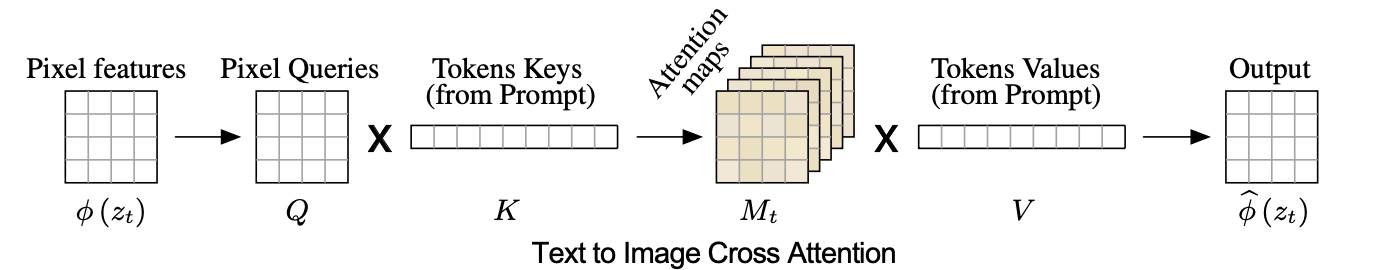
\includegraphics[width=.9\linewidth]{fig/cross_attention.png}
        \caption{Visual and textual embedding are fused using cross-attention layers that produce attention maps for each textual token. Figure source: \href{https://arxiv.org/pdf/2208.01626.pdf}{Hertz et al. (2022)}}
        \label{fig:crossattention}
    \end{figure}

\textbf{Latent Diffusion Model Pipeline:} 

The class \lstinline{MyLDMPipeline} implements and runs the entire pipeline of a latent diffusion model into which you will inject an implementation of Prompt-to-Prompt. 
Our latent diffusion pipeline implementation is based closely on the tutorial linked below; you should read this tutorial to better understand \lstinline{MyLDMPipeline}. 

\url{https://huggingface.co/docs/diffusers/main/en/using-diffusers/write_own_pipeline#deconstruct-the-stable-diffusion-pipeline}

The \lstinline{__init__} function of \lstinline{MyLDMPipeline} loads the different parts of the pre-trained model. The function \lstinline{generate_image_from_text} is the main entry point to  the entry point to this class which, as the name suggests, returns the generated image. It internally calls \lstinline{_generate_image_from_text} which performs the following key steps:

\begin{enumerate}
 
 \item Tokenization and Embedding of Prompts: The model's tokenizer converts both an empty string (to represent the unconditional generation case) and the actual text prompts into tokenized inputs. These tokenized inputs are then passed through a BERT-like model to obtain embeddings. The embeddings for the unconditional inputs and the text prompts are concatenated to serve as the context for the diffusion process. This ensures we can properly implement classifier-free guidance.
 
 \item Latent Space Initialization: You need to implement \lstinline{get_random_noise} that creates the initial values of the latents $\zv_T$. The latents must be of the correct dimension and will evolve into the final image through the diffusion process. You must implement support for the parameter \lstinline{same_noise_in_batch}. When \lstinline{same_noise_in_batch=False}, we follow the standard LDM setting for generating multiple images in parallel in a single batch: the noise is different for each sampled image. When running Prompt-to-Prompt however, we must set \lstinline{same_noise_in_batch=True}: in this setting, the noise is the same for each element of the batch. The first element of the batch will be the original image, and the other elements of the batch will be the prompt-edited images. This is useful because it isolates the effect of changes in the prompt from random differences in noise. This ensures that any differences in the final generated image are due solely to the change in the prompt.
 
  \item Diffusion Process: The core of the image generation happens here. For each timestep defined by \lstinline{num_inference_steps}, the function performs a diffusion step. This involves manipulating the latent space towards the desired outcome based on the context and the current timestep, under the guidance of the specified scale (\lstinline{guidance_scale}). The \lstinline{scheduler} is a \href{https://huggingface.co/docs/diffusers/en/api/schedulers/pndm}{PNDMScheduler} that enables the diffusion to run in fewer steps while still preserving the quality of the image (Note that the particular details of the schedule have no effect on your implementation of Prompt-to-Prompt, and we could have easily swapped in a different scheduler).

  \item Image Generation: After completing the diffusion steps, the final latent representation is converted into an image using the model's VQ-VAE (Vector Quantized Variational AutoEncoder). The image processor then converts the image to a PIL format (used by the Python Pillow library) for visualization. 

\end{enumerate}

\textbf{Cross Attention:} 

The LDM utilizes text prompts to influence the noise prediction at each diffusion step through cross-attention layers. Essentially, at each step $t$, the model predicts noise $\epsilon$ based on a noisy image $z_t$ and the text prompt's embedding $\psi(P)$ using a U-net architecture, leading to the final image $I = z_0$. The key interaction between image and text occurs in the noise prediction phase, where visual and textual embeddings are integrated via cross-attention layers. As illustrated in Fig.~\ref{fig:crossattention}, these layers generate spatial attention maps for textual tokens by projecting the image's deep features and text embedding into query ($Q$), key ($K$), and value ($V$) matrices through learned projections $\ell_Q, \ell_K, \ell_V$. The attention mechanism is formulated as:
\begin{equation}
M = \text{Softmax} \left( \frac{QK^T}{\sqrt{d}} \right),
\end{equation}
where $M_{ij}$ represents the influence of the $j$-th token's value on the $i$-th pixel, with $d_k$ being the dimensionality of the keys and queries. The output from cross-attention, $\phi_b(z_t) = MV$, updates the image features $\phi(z_t)$. Intuitively, $MV$ is a weighted average of $V$ based on the attention maps $M$, which are correlated to the similarity between Q and K. This process leverages multi-head attention to enhance expressiveness, concatenating the outcomes from parallel heads and refining them through an additional linear layer for the final output.

\textbf{Controlling Cross Attention:} 

Pixels are more attracted (correlated) to the words that describe them (you will visualize this when you run the notebook).
Building on the insight that cross-attention maps dictate the spatial layout and relationship between pixels and their corresponding descriptive words, Prompt-to-Prompt proposes a method to edit images while maintaining their original structure. By reusing attention maps $M$ from an initial generation with prompt $P$ in a subsequent generation with an altered prompt $P^*$, we can create an edited image $I^*$ that respects the original image's layout $I$.

We can define $DM(z_t, P, t, s)$ as the function for a single diffusion step $t$, outputting a noisy image $z_{t-1}$ and optionally an attention map $M_t$. We denote $DM(z_t, P, t, s)\{M \leftarrow \hat{M}\}$ to indicate the diffusion step with an externally supplied attention map $\hat{M}$ overriding the attention map \( M \), while maintaining the value matrix $V$ from $P$. The attention map generated with the edited prompt $P^*$ is $M_t^*$. The function $\text{Edit}(M_t, M_t^*, t)$ represents an editing operation on the attention maps of the original and edited prompts at step $t$. This general algo is written out in Fig.~\ref{fig:algo}.

    \begin{figure}[h!]
        \centering
        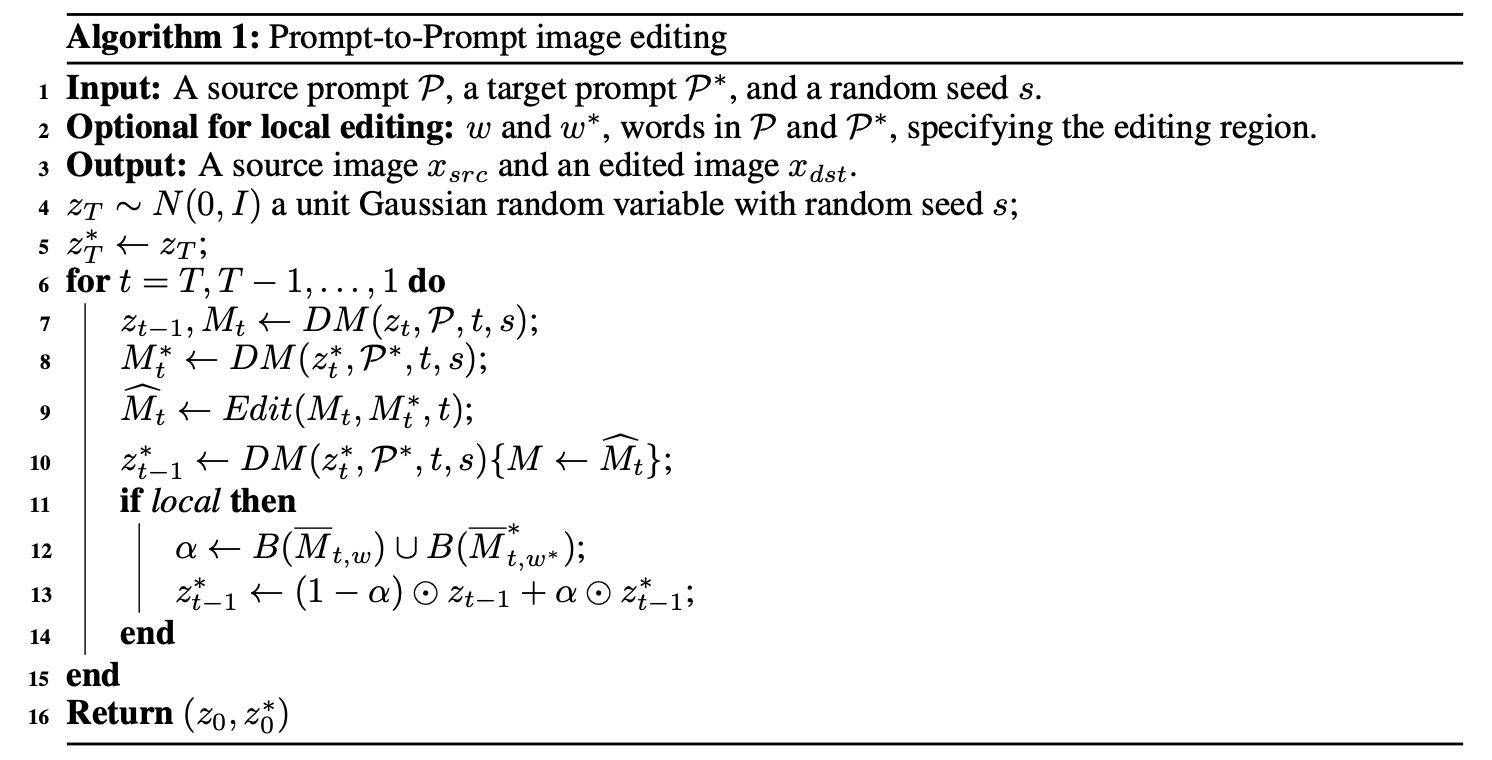
\includegraphics[width=.9\linewidth]{fig/algo.png}
        \caption{Algorithm: Prompt-to-Prompt image editing. Source: \href{https://arxiv.org/pdf/2208.01626.pdf}{Hertz et al. (2022)}. Note that \textit{local} is always False in our implementation. }
        \label{fig:algo}
    \end{figure}

\textbf{Word Swap:} 

While Prompt-to-Prompt can be used for various different types of edit operations on the prompt, we will focus exclusively on word swapping, e.g., \( P\) = “a
big bicycle” to \( P^* \)= “a big car”.

For word swapping, we inject the attention maps of the source image into the generation by the modified prompt. We work with the \lstinline{MySharedAttentionSwapper} class, where you will initialize a mapper tensor as \lstinline{self.mapper}, and with the \lstinline{MyCrossAttentionClass}. It is designed to facilitate the replacement of tokens in the cross-attention map and should be used to reassign attention from the old tokens to the new ones (dive into the code base to see what exactly it does and also refer to the section on Replacement Mapper). You will implement:

\begin{itemize}
 
\item one line of code in \lstinline{swap_attention_probs(...)} in the \lstinline{MySharedAttentionSwapper} class where you swap out the existing attention with the \lstinline{self.mapper}. Here you want to use the mapper matrix to get the swapped attention probabilities for each of the modified prompts. Note that the self.mapper matrix contains all of the mapper matrices stacked together. This can be done cleanly in one line of code using \lstinline{einsum}. 
  
\item \lstinline{forward} method of the \lstinline{MyCrossAttentionClass}: In this method you need to initialize and implement the attention mechanism, which means you need to initialize your query, key and value tensors, and use them to calculate the attention probabilities. Once the prompt-to-prompt attention swapping is done, you need to calculate the hidden states and apply the linear projection, dropout and if required, add the residual connection. \\
Some functions that might come in handy are:
\begin{itemize}
    \item \lstinline{self.attn.to_q}, \lstinline{self.attn.to_k} and \lstinline{self.attn.to_v}: these are linear transformations that project the input into query, key, and value vectors, which are used to compute attention scores and weighted outputs in the attention mechanism.

    \item \lstinline{}
    \lstinline{self.attn.head_to_batch_dim()}. This function takes in an attention matrix and reshapes it to facilitate multi-headed attention.

    \item 
    \lstinline{self.attn.get_attention_scores}. Takes in the query, key, and attention mask to return the attention probabilities.

    

    \item \lstinline{torch.bmm}: performs a batch-wise matrix multiplication of two 3D tensors. Specifically, if you have tensors of shape (b, n, m) and (b, m, p), \lstinline{torch.bmm} multiplies each pair of matrices in the batch (of size b) to produce a new tensor of shape (b, n, p). This can be helpful to compute the output of the attention mechanism (multiplying the attention weights by the values)

    \item 
\lstinline{self.attn.batch_to_head_dim()}. Takes in a multi-headed attention matrix and reshapes it to a single tensor with the original dimensions.

\item 
\lstinline{self.attn.to_out[0]}. The linear projection layer to be applied to the hidden state.

\item 
\lstinline{self.attn.to_out[1]}. Dropout layer to be applied to the output of the linear projection layer.

\item 
\lstinline{self.attn.rescale_output_factor}
\end{itemize}



\end{itemize}


\textbf{Replacement Mapper:}

In the function \lstinline{get_replacement_mapper}, we return the stacked PyTorch tensor containing all the mapping matrices, where each matrix corresponds to the mapping from the first prompt to one of the subsequent prompts. It calls upon \lstinline{get_replacement_mapper_} (which you will implement) that splits both input strings \lstinline{x} and \lstinline{y} into words and constructs a mapping matrix of size \lstinline{max_len} $\times$ \lstinline{max_len}, with values in $[0,1]$ indicating the matching between the changing word in the input prompt and the corresponding word in the modification prompt.

Remember, there are 4 cases to consider: 1-to-1, 1-to-n, n-to-1, and n-to-m. Refer to the recitation for more details on what this means. Your code should accurately detect which case you are in and construct the appropriate mapper matrix.

(Hint: For most things in PyTorch we avoid for loops, but you needn't do so here. Since this method is only called once during initialization, \lstinline{for} loops are fine.)

(Hint: The helper function \lstinline{get_word_inds} will be useful here)

\textbf{Evaluation:} 

We ask you to run the notebook to get the visualizations once you complete filling in the needed functions. You will be visualizing replacement edit and local editing results.

\clearpage

\uplevel{\subsection*{Empirical Questions}}

\begin{parts}

\part[1] \textbf{Short answer:} Print out the structure of the UNet model by calling \lstinline{print(pipe.unet)}. Notice that within the \textit{up} and \textit{down} transformer blocks (\lstinline{BasicTransformerBlock}), there are two attention layers: one is named \lstinline{attn1} and the other \lstinline{attn2}. Which of these two is self-attention and which is cross-attention? \textbf{Briefly justify your answer based on the printout of the model.}

\begin{answer_box}[title=,height=8cm, width=15cm]
\end{answer_box}
  

\uplevel{The questions below refer directly to the section headers of the Colab notebook in \lstinline{run_in_colab.ipynb}.}


\part[2] Paste the results from the section `Baseline: Different Initial Noise for Each Prompt'
\label{question-baseline}

[Expected runtime on Colab T4: 30s]

\begin{answer_box}[title=,height=8cm, width=15cm]
  \end{answer_box}
  
\part[2] Paste the results from the section `Same Initial Noise for Each Prompt'
\label{question-a}

[Expected runtime on Colab T4: 30s]

\begin{answer_box}[title=,height=8cm, width=15cm]
  \end{answer_box}

\part[1] Briefly explain how your results from Question \ref{question-baseline} differ from your results in Question \ref{question-a}?

\begin{answer_box}[title=,height=4cm, width=15cm]
\end{answer_box}

\clearpage

\part[2] Paste the results from the section `Prompt-to-Prompt: Word Swap'
\label{question-b}

[Expected runtime on Colab T4: 30s]

\begin{answer_box}[title=,height=8cm, width=15cm]
  \end{answer_box}


\part[1] Briefly explain how your results from Question \ref{question-a} differ from your results in Question \ref{question-b}?

\begin{answer_box}[title=,height=4cm, width=15cm]
\end{answer_box}

\clearpage


\part[2] Paste the results from the section `Prompt-to-Prompt: Modify Cross-Attention Injection'
\label{question-c}

[Expected runtime on Colab T4: 30s]

\begin{answer_box}[title=,height=15cm, width=15cm]
  \end{answer_box}


\part[2] How do your results in Question \ref{question-c} vary as you change the cross attention parameters? 

\begin{answer_box}[title=,height=4cm, width=15cm]
\end{answer_box}

\clearpage


\part[2] Paste the results from the section `Prompt-to-Prompt: Modify Self-Attention Injection'
\label{question-d}

[Expected runtime on Colab T4: 30s]

\begin{answer_box}[title=,height=15cm, width=15cm]
  \end{answer_box}


\part[2] How do your results in Question \ref{question-d} vary as you change the self attention parameters? 

\begin{answer_box}[title=,height=4cm, width=15cm]
\end{answer_box}

\clearpage


\part[2] Paste the results from the section `Prompt-to-Prompt: Single-Token to Multiple-Token Word Swap'
\label{question-e}

[Expected runtime on Colab T4: 30s]

\begin{answer_box}[title=,height=8cm, width=15cm]
  \end{answer_box}


\part[2] Paste the results from the section `Prompt-to-Prompt: Multiple-Token to Single-Token Word Swap'
\label{question-f}

[Expected runtime on Colab T4: 30s]

\begin{answer_box}[title=,height=8cm, width=15cm]
  \end{answer_box}

\clearpage


\part Define your own base prompt and three prompt edits (i.e. something other than the examples provided in the \lstinline{.ipynb}) and run them through Prompt-to-Prompt.

\begin{subparts}

\subpart[1] Report the prompts and any hyperparameters that you used.
\begin{answer_box}[title=,height=8cm, width=15cm]
  \end{answer_box}

\subpart[2] Paste the resulting images below.
\begin{answer_box}[title=,height=8cm, width=15cm]
  \end{answer_box}
     
\end{subparts}


  
\end{parts}


\clearpage
\sectionquestion{Code Upload}

\begin{parts}

\part[0] Did you upload your code to the appropriate programming slot on Gradescope? \\
\emph{Hint:} The correct answer is `yes'.

    \begin{checkboxes}
     \choice Yes 
     \choice No
    \end{checkboxes}

For this homework, you should upload only \lstinline{prompt2prompt.py}.

\end{parts}

\newpage
\sectionquestion{Collaboration Questions}

\begin{parts}

\uplevel{After you have completed all other components of this assignment, report your answers to these questions regarding the collaboration policy. Details of the policy can be found in the syllabus.}

    \part[1] Did you collaborate with anyone on this assignment? If so, list their name or Andrew ID and which problems you worked together on.

        \begin{answer_box}[title=,height=3cm, width=15cm]
        \end{answer_box}

    
    \part[1] Did you find or come across code that implements any part of this assignment? If so, include full details.
        \begin{answer_box}[title=,height=3cm, width=15cm]
        \end{answer_box}
\end{parts}
\end{questions}


\end{document}
